\documentclass[11pt, paper=a4]{scrartcl}

% CONFIG
\newcommand{\exptitle}{Optical pumping}       % long name of experiment 
\newcommand{\exptitleshort}{Optical pumping} % short name of experiment
\newcommand{\expdate}{11.04.2016}           % date of experiment
\newcommand{\exptutor}{Dominik Schomas}

% PACKAGES + MODIFICATIONS
%\usepackage[ngerman]{babel} %standard language stuff
\usepackage[T1]{fontenc}
\usepackage[utf8]{inputenc}
\usepackage{textgreek}

\usepackage{soul} %better underline
\setul{2pt}{.4pt} %set underline 2 pts below text and thickness to .4pt

\usepackage[fleqn]{amsmath}  % math
\usepackage{amssymb}
\usepackage[]{units} %units package for fractions
\usepackage[amssymb]{SIunits} %units package for sinunits

\usepackage{graphicx} %graphics
\usepackage{float} 

\usepackage[automark,headsepline]{scrlayer-scrpage} %headings
\pagestyle{scrheadings}
\ihead{\exptitleshort}
\ohead{\pagemark}
\cfoot{}

\usepackage{hyperref}
\hypersetup{
    unicode=true,          % non-Latin characters in Acrobat’s bookmarks
    pdftoolbar=true,       % show Acrobat’s toolbar?
    pdfmenubar=true,       % show Acrobat’s menu?
    pdffitwindow=false,    % window fit to page when opened
    pdfstartview={FitH},   % fits the width of the page to the window
    pdfnewwindow=true,     % links in new window
    colorlinks=true,       % false: boxed links; true: colored links
    linkcolor=blue,       % color of internal links (change box color with linkbordercolor)
    citecolor=green,       % color of links to bibliography
    filecolor=magenta,     % color of file links
    urlcolor=blue          % color of external links
}

\usepackage[labelfont=bf]{caption} % bold captions

\usepackage{chngcntr} % change behaviour of counters in different environments
\counterwithin{figure}{section}  % number figures per section
\numberwithin{equation}{section} % number equations per section
\numberwithin{table}{section}    % number tables per section

\usepackage{enumerate} % better way to config enumerates

\setcounter{tocdepth}{2} % table of contents depth

\setlength{\parindent}{0pt} % no indent on new paragraph

\usepackage{pdfpages} % include pdf files

\usepackage[nottoc,numbib]{tocbibind} % bibliography in TOC

% NEW COMMANDS
\newcommand{\refeq}[1]{\overset{\text{\eqref{#1}}}{=}}

% DOCUMENT SETTINGS

\title{\exptitle}
\subtitle{}
\author{}
\date{\expdate}

% DOCUMENT
\begin{document}

\hypersetup{pageanchor=false} %stop page numbering (hyperref) to prevent for double page numers
\newcommand{\HRule}{\rule{\linewidth}{0.5mm}}
\begin{titlepage}
\begin{center}
  \textsc{\Large Fortgeschrittenen Praktikum II }\\[0.5cm]
  \HRule \\[0.4cm]
  { \huge \bfseries \exptitle}\\
  \HRule \\[0.5cm]
  \large \expdate\\[0.5cm]  
  Benjamin Winkelmann \\
  Peter Spalthoff \\
  \vspace{10pt}
  \large 
  Tutor: \exptutor \\[3cm]
  \vfill
  \normalsize
\end{center}
\end{titlepage}
\thispagestyle{empty}



\pagenumbering{Roman}
\setcounter{page}{1}


\section{Abstract}
Optical pumping between Zeeman states of rubidium isotopes $^{87}$Rb and $^{85}$Rb that are split up by well controlled magnetic fields allows for the precise calculation of the earths magnetic field, hyperfine constants $A$ of the two isotopes as well as the relaxation time of the polarized states. The resulting hyperfine constants were calculated as
\begin{align}
	A_{^2S_{\nicefrac{1}{2}}}(^{87}Rb)&=\unit{(14.61\pm0.13)}{\micro\electronvolt}\\
	A_{^2S_{\nicefrac{1}{2}}}(^{85}Rb)&=\unit{(4.50\pm0.08)}{\micro\electronvolt}\\
	A_{^2P_{\nicefrac{1}{2}}}(^{87}Rb)&=\unit{(1.52\pm0.18)}{\micro\electronvolt}
\end{align}
The hyperfine constant $A_{^2P_{\nicefrac{1}{2}}}(^{85}Rb)$ could not be calculated since the relevant peaks could not be separated with the set-up.
The earths' magnetic field components were calculated to be
\begin{align}
	B_v&=\unit{(37.1\pm1.4)}{\micro T}\\
	B_h&=\unit{(2.36\pm 0.21)}{\micro T}
\end{align}
Of the two methods used to calculate the relaxation times, only the Dehmelt method produced a reasonable result for the relaxation time:
\begin{equation}
T_R=\unit{(4.8\pm1.5)}{ms}
\end{equation}
\tableofcontents

\newpage
\listoffigures
\thispagestyle{empty}

\newpage
\hypersetup{pageanchor=false} %stop page numbering (hyperref) to prevent for double page numers

\clearpage
\pagenumbering{arabic}
\setcounter{page}{1}

\section{Goal of the experiment}
In this experiment, the process of optical pumping will be used to precisely measure properties of Rubidium atoms such as the hyperfine constant $A$ via absorption measurements. In addition to that, relaxation times of the induced pumped states as well as external magnetic fields will also be measured by observing the effect of magnetic fields, applied through Helmholtz coils, high frequency radio waves and variations in the laser intensity.
\section{Physical principles}
\subsection{Hyperfine structure and Zeeman splitting}
This section is based on the detailed elaborations in \cite{staatsex}.\\
The fine structure levels of the atomic spectrum, which splits the basic levels into sub-levels due to spin-orbit interaction, can be shown to be split into even finer levels, whose energetic distances are roughly three orders of magnitude smaller than those of the fine structure. This is called the 'hyperfine structure' and is mainly caused by the interaction of the nuclear magnetic dipole and quadrupole moment and the magnetic field of the shell electrons. Its structure for the two Rubidium isotopes that are used in this experiment can be seen in figure \ref{fig:hyperfinestructure}.\\

As the nucleus is charged and, expressed as the nuclear spin $\vec{I}$, has angular momentum, it also has a magnetic moment, which is $\vec{\mu}_I=\frac{g_I\mu_K}{\hbar}\vec{I}$, where $g_I$ is the g-factor of the nucleus and $\mu_K$ is the nuclear magneton. 

With the total angular momentum of the electrons $\vec{J}$, the total angular momentum of the atom can be written as

\begin{equation}
\vec{F}=\vec{J}+\vec{I},\qquad \lvert I-J\rvert\le F \le I+J
\end{equation}

The energy difference between hyperfine structure levels can then shown to be

\begin{equation}
\Delta E_{HFS}=-\vec{\mu}_I\cdot\vec{B}_J=\frac{A}{2}(F(F+1)-J(F+1)-I(I+1))
\end{equation}

where $A=\frac{g_I\mu_KB_J}{\sqrt{J(J+1)}}$ is the hyperfine constant. Neighboring levels thus have an energy difference of

\begin{equation}
\Delta E_{HFS}(F+1)-\Delta E_{HFS}(F)=A(F+1)
\end{equation}

\begin{figure}[H]
\centering
\includegraphics[width=1.0\linewidth]{graphics/hyperfinestructure}
\caption[Hyperfine structure of Rubidium]{The hyperfine structure of the two isotopes of Rubidium used in the experiment. An exemplary Zeeman splitting is included as well. \cite{staatsex}}
\label{fig:hyperfinestructure}
\end{figure}


\subsection{Optical pumping}
\subsection{Larmor precession of the spin}
\subsection{Relaxation processes}
\subsection{The laser diode}


\section{Experimental set-up}
\begin{figure}[h]
\centering
\includegraphics[width=1.0\linewidth]{graphics/generalsetup}
\caption[Basic experimental set-up]{Basic set-up of the experiment. For the various tasks, parts can be placed onto the optical bench. The glass cell can be removed from the central unit. \cite{anleitung} (modified)}
\label{fig:general setup}
\end{figure}
At the core of the experimental set-up is the glass cell with the Rubidium vapor and the buffer gas. It can be taken in and out of the central unit, which in turn houses four sets of Helmholtz coils. Another such pair is directly attached to the casing of the glass cell, along with a radio frequency generator and an appropriate frequency measuring device.\\

\textbf{A laser diode} provides coherent light in the energy range needed to pump the desired hyperfine state of the Rubidium atoms in the glass cell. Laser diodes send out linearly polarized light with a small spectral width. Frequency and intensity vary with the temperature of the diode as well as the current running through it, which is why the diode is kept at constant temperature using a Peltier element. For the diode to start emitting light, a certain current threshold has to be reached. From then on, the intensity depends linearly on the current if temperature is kept constant. However, mode jumps at certain currents disturb the linearity. Mode jumps occur when the number of standing waves in the resonator changes. Measurements need to be taken in areas that do not include such jumps.\\

The beam is collimated by a lens before passing through other optical elements and, after passing through the central unit, is refocused onto a photo-diode. This can be seen in figure \ref{fig:general setup}. The output of the diode is amplified and can then be observed on an oscilloscope, which in turn can be read out by a computer to produce analyzable data.\\ 

The set-up varies greatly from one part of the experiment to another and will thus be explained in detail in the appropriate sections.


\section{Characterization of the laser diode}
For later measurements, it is important to determine the range of supply current in which the diode intensity increases linearly without mode jumps occurring. The gas cell is taken out of the central unit for this part of the experiment. \\

After turning on the peltier element, a few minutes should pass before measurements are started to allow the diode to thermalize. Measurements were taken at $T=\unit{34.3}{\degree}$.\\
Since the photo diode saturated for laser diode currents upwards of $I_L=\unit{65}{mA}$, a neutral filter (D2,6) is used to limit the intensity so that the photo diode barely does not reach saturation.

The intensity of the diode is now measured at supply currents between $\unit{0-90}{mA}$. The results can be seen in figure \ref{fig:characterization}. The threshold current is roughly $\unit{51.6}{mA}$, followed by the linear domain until mode jumps occur at around $\unit{72}{mA}$ to $\unit{82}{mA}$. 
\begin{figure}[htb]
\centering
\includegraphics[width=1.0\linewidth]{graphics/characterization}
\caption[Characteristic curve of the laser diode]{The characteristic curve of the laser diode for supply currents up to $\unit{90}{mA}$. A mode jump can clearly be seen in the uper right corner.}
\label{fig:characterization}
\end{figure}







\section{Spectroscopy of the hyperfine structure}
\subsection{Set-up and procedure}
\begin{figure}[htb]
	\includegraphics[width=1.0\linewidth]{graphics/calibrationsetup}
	\caption[Experimental set-up for the Calibration]{Experimental set-up for the calibration measurements. An etalon is placed after the left lens and can be removed for the HFS-spectrum measurement.\cite{anleitung}}
	\label{fig:calibration setup}
\end{figure}
\subsubsection*{Laser scan-rate}
A Fabry-Pérot-Interferometer (etalon), which is a set of parallel, almost completely reflecting surfaces facing each other, is used to gauge the diode. The intensity at the photo diode will be drastically dampened unless the laser wavelength allows for constructive interference to occur between the surfaces. The wavelengths at which light passes the interferometer are thus equidistant.\\

The diode current is then modified with a saw-tooth voltage, which is also used to trigger the oscilloscope(see figure \ref{fig:calibration setup}). It is important to measure the scan-rate in a range of diode currents where the intensity response is linear and where the HFS-spectrum is actually visible (see next section). To get a solid calibration, at the very least 3 etalon peaks are necessary. These two factors have to be taken into consideration when choosing the measurement interval.\\ 

Figure \ref{fig:bendincurve} shows a bend in the diode current. Such areas need to be avoided when taking measurements, as they would lead to non-equidistant peaks in the etalon spectrum and unnecessarily complicate data analysis.
\begin{figure}
	\centering
	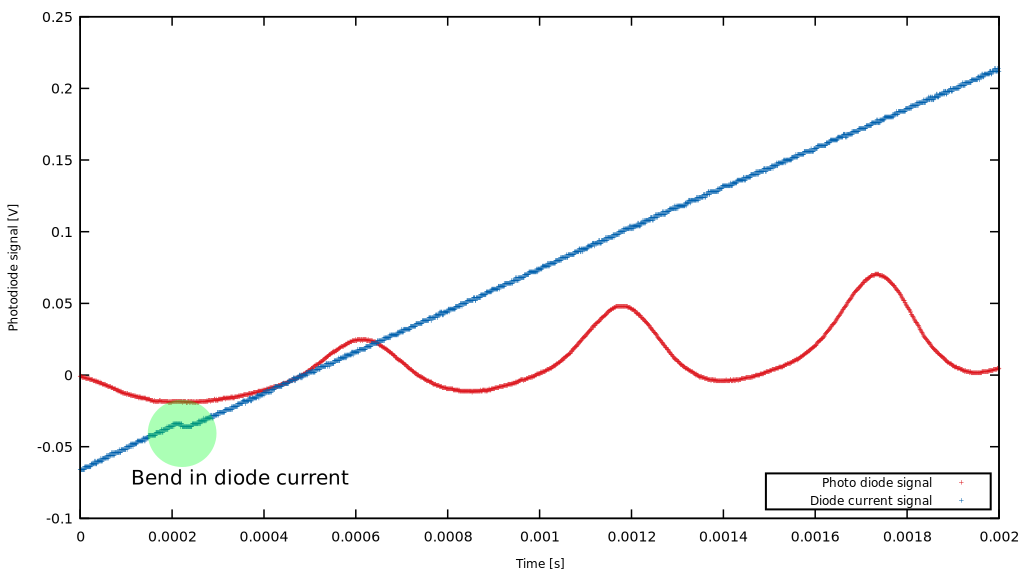
\includegraphics[width=1.0\linewidth]{graphics/bendincurve}
	\caption[Bend in modulating current]{In the bottom left corner, a clear bent in the diode current can be seen. These measurements were not used, a better current range was chosen instead.}
	\label{fig:bendincurve}
\end{figure}
The base current for the measurements was $I_L=\unit{(58.5\pm0.1)}{mA}$, where the uncertainty is the digit error of the multimeter ELTELEC, for which no data sheet was available. The temperature remained at $T=\unit{34.3}{\degree}$. The resulting intensity distribution can be seen in figure \ref{fig:etalon_fit}.

\subsubsection*{The HFS-spectrum}
The etalon is removed for this measurement and the exact same current modulation of the laser current as has been used for the scan-rate measurements will be used here as well. As the intensity increases with increasing diode current, the spectrum would have a linear offset. This can be counteracted by inverting the photo diode signal and adding the diode current signal to it. An additional cosmetic advantage of this is that the peaks are then positive.


\subsection{Data analysis}
\subsubsection*{Laser scan rate}
\begin{figure}[htb]
\centering
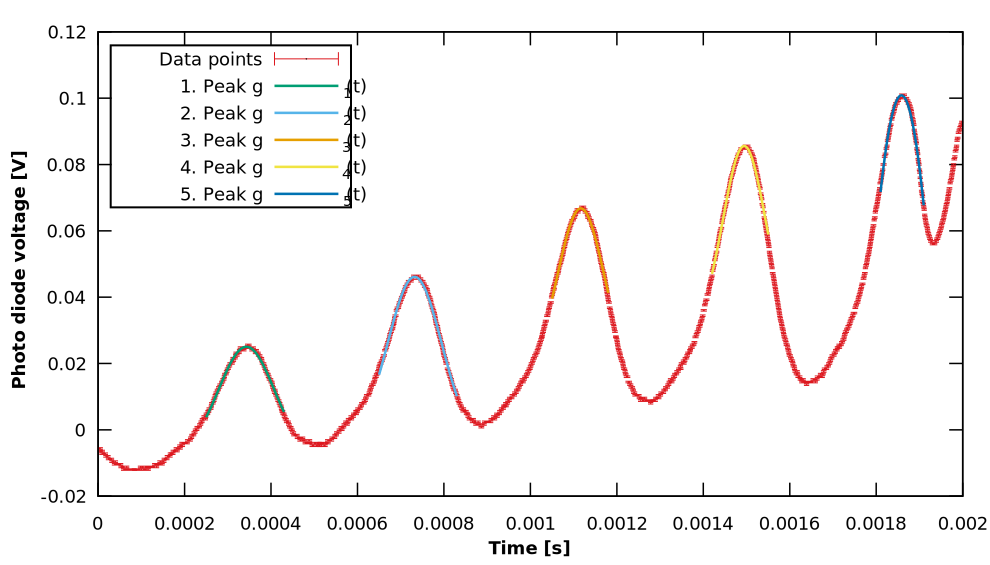
\includegraphics[width=1.0\linewidth]{graphics/etalon_fit}
\caption[Etalon peaks]{Results of the etalon calibration measurements. The rightmost peak is actually the same as the one on the left of it, as the saw-tooth reaches its peak between the two.}
\label{fig:etalon_fit}
\end{figure}
In figure \ref{fig:etalon_fit}, it has to be noted that the saw-tooth voltage reaches its maximum between the rightmost peak and the one on the left of it, meaning that these two actually belong to the same frequency. The rightmost peak is thus ignored for the calibration.\\
Gauss functions with a constant offset of the form
\begin{equation}
	g_i(t)=a_i*e^{-\frac{(t-t_{0,i})^2}{2*\sigma_i^2}}+c_i
	\label{eq:gaussfit}
\end{equation}
and a linear offset function $l(t)=b*t+c$ were used. 
The results for the peak positions $t_{0,i}$ can be seen in figure \ref{fig:ethalon_linearfit}. As the linear fit shows, these peaks are equidistant as expected with the time distance between peaks being $b=\unit{(0.379\pm0.003)}{ms}$. The nominal distance between two peaks is $\Delta_{FSR}=\unit{(9924\pm30)}{MHz}$. With these two values, the scan rate $r$ of the laser can be calculated as
\begin{equation}
	r=\unit{(26.17\pm 0.22)}{\frac{GHz}{ms}}
\end{equation}

\begin{figure}[htb]
\centering
\includegraphics[width=1.0\linewidth]{graphics/ethalon_linearfit}
\caption[Lienear fit on etalon peak positions]{Linear fit on the etalon peak positions.}
\label{fig:ethalon_linearfit}
\end{figure}

\subsubsection*{HFS-spectrum}
Only 6 of the expected 8 peaks (see fig. \ref{fig:hfslevels}) are visibly separated here. It is reasonable to assume that the peaks that were not separable are those of the transitions $^{85}$Rb F:3-2 and $^{85}$Rb F:3-3 as well as $^{85}$Rb F:2-2 and $^{85}$Rb F:2-3. This also means that the hyperfine constant for the $^2S_{\nicefrac{1}{2}}$ of $^{85}$Rb cannot be calculated with these measurements.
Gauss functions like those in equation \ref{eq:gaussfit} were used for the individual peaks. However, for the peaks that overlap, as sum of the two functions was used. For all fits, both a linear function and a constant were added and the total sum fitted to the data. The fit function for the last three peaks for example was
\begin{equation}
I_{4-6}(t)=g_4(t)+g_5(t)+g_6(t)+b\cdot t+c
\end{equation}
Table \ref{tb:HFSresults} lists the result of the fits as well as the frequency distances $\nu_{i}$ of the i-th peak to the first peak, which was arbitrarily chosen as a point of comparison. The differences between the peaks were compared to those expected (see fig. \ref{fig:hfslevels}) and the transitions were attributed accordingly. The uncertainties of the peak center times stem from the fits.\\

\begin{figure}[htb]
	\centering
	\includegraphics[width=1.0\linewidth]{graphics/HFS_fits}
	\caption[The HFS-spectrum]{The HFS-spectrum with fits to the individual peaks. The signal is negative since it was inverted.}
	\label{fig:HFS_fits}
\end{figure}


With these distances known and the help of equation \ref{eq:hfslevels}, the hyperfine constants can be calculated. For $A_{^2P_{\nicefrac{1}{2}}}(^{87}Rb)$, the calculation is
\begin{equation}
	A_{^2P_{\nicefrac{1}{2}}}(^{87}Rb)=h\cdot\frac{\nu_8-\nu_7}{F+1}=\unit{(1.52\pm0.18)}{\micro\electronvolt}
\end{equation}
where $F=1$ is the total angular momentum of the atom in the state that the transitions have in common. This value encloses the literature value $A_{^2P_{\nicefrac{1}{2}}}(^{87}Rb)=\unit{1.692}{\micro\electronvolt}$ \cite{corney} in its $1\sigma$ interval.\\
The other two calculable hyperfine constants are
\begin{align}
	A_{^2S_{\nicefrac{1}{2}}}(^{87}Rb)&=h\cdot\frac{\nu_8-\nu_2}{F+1}=\unit{(14.61\pm0.13)}{\micro\electronvolt}\\
	A_{^2S_{\nicefrac{1}{2}}}(^{85}Rb)&=h\cdot\frac{\nu_{5/6}-\nu_{3/4}}{F+1}=\unit{(4.50\pm0.08)}{\micro\electronvolt}
\end{align}
which both place their respective literature values $A_{^2S_{\nicefrac{1}{2}}}(^{87}Rb)=\unit{14.13}{\micro\electronvolt}$ and $A_{^2S_{\nicefrac{1}{2}}}(^{85}Rb)=\unit{4.185}{\micro\electronvolt}$ outside of their $3\sigma$ intervals. While the distance between the first and eigth peak of the spectrum is within $1\sigma$ of the expected value, the spectrum in between seems to be somewhat distorted. As we can also not separate the third and forth as well as the fifth and sixth peak, which are both more than 5 times further apart than the largest statistical error that was calculated, one has to assume that either the statistical errors are vastly underestimated or that there is a systematic error that is unaccounted for. Such a systematic error could be a not completely linear current modulation or the effect of the etalon not being placed perfectly perpendicular to the beam.

\begin{table}\centering
	\begin{tabular}{@{}llllllll@{}}
		\toprule
		&Peak $i$ &$t_0$ [ms]&$s_{t_0}$ $\unit{}{[\micro s]}$ &$\Delta\nu_{i}$ [GHz]&$s_{\Delta\nu_{i}}$ [GHz]&$\Delta\nu^{theo}_{i}$ [GHz]&Transition\\
		\midrule
		&1&0.104&0.18&-&-&-&$^{87}$Rb F:1-2\\
		&2&0.129&0.92&0.648&0.005&0.82&$^{87}$Rb F:1-1\\
		&3/4&0.215&0.05&2.905&0.024&2.66 / 3.02&$^{85}$Rb F:2-2/3\\
		&5/6&0.340&0.03&6.17&0.05&5.70 / 6.06&$^{85}$Rb F:3-2/3\\
		&7&0.371&0.06&6.98&0.06&6.83&$^{87}$Rb F:2-2\\
		&8&0.399&0.06&7.71&0.06&7.65&$^{87}$Rb F:2-1\\	
		\bottomrule
	\end{tabular}
	\caption[HFS peaks fit results]{Fit results of the Gauss fits on the HFS spectrum. The frequency calibration was used to calculate the frequency differences to the preceding peak. Theoretical values were taken from \cite{staatsex}.}
	\label{tb:HFSresults}
\end{table}


\newpage
\begin{thebibliography}{9}
	\bibitem{staatsex}
	Baur, Clemens. "Einrichtung des Versuchs \emph{Optisches Pumpen mit Laserdioden}."
	Zulassungsarbeit. Freiburg 1997
	\bibitem{anleitung}
	"Instructions for the experiment \emph{Optical Pumping}." Albert-Ludwig University Freiburg. Freiburg 02.2016
	\bibitem{happer}
	Happer, William. "Optical pumping."
	\ul{Reviews of Modern Physics} 44.2 (Apr. 1972): 170-238
\end{thebibliography}


\end{document}
